\subsection{DNS}
\subsubsection{DNS Provisions}
\textbf{Effeciency} is, amongst other things, achieved in the DNS Message Format. It allows the serving of multiple RRs 
in a single request, meaning that any DNS request will either lead you to the target you're looking for (A/CNAME/MX), or
provide you with further NS records to ask another DNS server for the answer. In addition, \textbf{cacheing} is an important
strategy in maintaining the effeciency of DNS requests. Requests will drive you toward the correct DNS servers that
houses the information you need, hopefully localized near the client. Fault tolerance and scalability are provided by IP-reordering
on each new request, along with the ability to forward to a number of different available DNS servers to serve the request. From the ground
up, DNS is built as a distributed name-service provider, not a centralized one.

\subsubsection{DNS Lookup and Format}
\textbf{Part 1:}\\
CNAME records allow you to provide any number of alias hostnames, allowing you to have f.ex ftp.myserver.com and webmail.myserver.com
that both point to the same IP address(es). In addition, a single CNAME record can contain a set of IP addresses. DNS provides simple 
load-balancing through re-ordering the IP addresses that it returns, on each subsequent request. This is a primitive form of round-robin, 
and will in most cases mean that a different server is contacted by the requester, since most services will simply pick the first IP address
provided. 

\noindent \textbf{Part 2:}\\
A recursive query is a query for someone else to perform a lookup on your behalf; such as a client requesting a DNS entry, from a local DNS server.
This entails further, \textbf{recursive} requests, hence the name.

An iterative query is one amongst many \textbf{iterations} of queries sent out from a single machine, hence the name. This could f.ex be the
local DNS server, which has just been sent a recursive query by a client. It will then ask a root-level DNS server for the right TLD DNS, the
TLD DNS for one or several correct authoritative DNS servers, and then finally the authoritative DNS server for the CNAME/A/MX records. It may
be that when the local DNS server asks the root-level server for the right TLD, that it is simply passed another name-server to ask the same
thing, and not a direct answer.

A typical DNS request will follow the above format, but does not have to. Recursive requests are very important for caching strategies, and
to help balance load on DNS servers.

\noindent \textbf{Part 3:}\\
\begin{table}
\begin{tabular*}{1\textwidth}{| c | c |}
	\hline
	NS entry & (com., a.gtld-servers.net, NS, 172800)\\
	\hline
	A entry & (a.gtld-servers.net, 192.5.6.30, A, 172800)\\
	\hline
	CNAME entry & (www.grooveshark.com, grooveshark.com, CNAME, 2302)\\
	\hline
\end{tabular*}
\caption{DNS resource-record examples}
\label{tbl:rrexamples}
\end{table}

Figure \ref{fig:dnsreq} demonstrates an example DNS request sequence, in which a recursive DNS request is first sent to ns2.censurfridns.dk,
followed by iterative requests to a root-level and TLD-level DNS servers. The total number of DNS messages sent in this example is 8.

Response 3 (From a.root-servers.net to ns2.censurfridns.dk) contains a set of NS entries in its AUTHORITY section. However, in order to look them
up, the recursive requester needs the actual IP to find those name servers on. This information is contained in the ADDITIONAL section, as A
records. 

Response 5 (From a.gtld-servers.net to ns2.censurfridns.dk) contains yet-another set of NS entries in the AUTHORITY section, and their A records
in the ADDITIONAL section. These yield the Authoritative name-servers that can tell more about grooveshark.com.

Response 7 (From ns1.grooveshark.com to ns2.censurfridns.dk) contains, beyond the same set of name servers belonging to grooveshark, the answer
requested by ns2.censurfridns.dk, namely the A record for grooveshark.com. This is the answer that the requesting client is looking for, and
is passed back to it in response 8.

Table \ref{tbl:rrexamples} showcases some example resource-records from this DNS request sequence.

\begin{figure}[htb]
\centering
\setlength\fboxsep{0pt}
\setlength\fboxrule{0.5pt}
\fbox{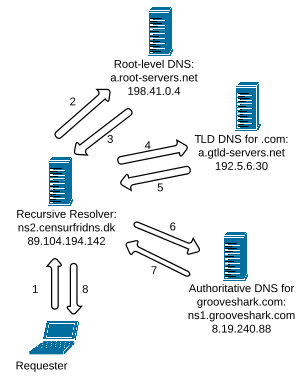
\includegraphics[scale=1]{dnsreq.png}}
\caption{DNS Request for grooveshark.com}
\label{fig:dnsreq}
\end{figure}

\subsubsection{}
